% Paper 7. IEEE conference layout emulated with article + mathptmx (official IEEEtran.cls not available offline;
% on Overleaf, replace the first block with \documentclass[conference]{IEEEtran}).
\documentclass[10pt,twocolumn,letterpaper]{article}
\usepackage[top=0.75in,bottom=1in,left=0.625in,right=0.625in,columnsep=0.25in]{geometry}
\usepackage{mathptmx}
\usepackage[T1]{fontenc}
\usepackage{amsmath,amssymb,amsthm}
\usepackage{graphicx,booktabs,multirow,xcolor}
\usepackage{titlesec,abstract,balance,stfloats}
\usepackage[hidelinks]{hyperref}
\usepackage[font=footnotesize,labelfont=bf,labelsep=period]{caption}
\renewcommand{\thesection}{\Roman{section}}
\renewcommand{\thesubsection}{\Alph{subsection}}
\titleformat{\section}{\centering\normalsize\scshape}{\thesection.}{0.5em}{}
\titleformat{\subsection}{\normalsize\itshape}{\thesubsection.}{0.5em}{}
\titlespacing*{\section}{0pt}{8pt}{4pt}
\titlespacing*{\subsection}{0pt}{6pt}{3pt}
\renewcommand{\abstractnamefont}{\normalfont\small\bfseries\itshape}
\renewcommand{\abstracttextfont}{\normalfont\small\bfseries}
\setlength{\absleftindent}{0pt}\setlength{\absrightindent}{0pt}
\newtheorem{proposition}{Proposition}
\newcommand{\Q}[1]{\textbf{Q#1}}
\newcommand{\Fs}{F_{\mathrm{stuck}}}

\title{\Large\bfseries Is a Little Slip Worth It? Certified Fast Lifting for Residual\\ Policies Under a Static-to-Kinetic Friction Drop}
\author{Clement Aidoo\\ \small CANLABS, Ghana \quad \texttt{clement.aidoo@canlabs.org}\\
\small Code, data and protocol: \url{https://github.com/CAN-Aidoo/lift-shield}}
\date{}

\begin{document}
\maketitle

\begin{abstract}
A gripper that lifts an object of unknown weight and friction must choose how hard to squeeze and how fast to move.
Squeezing less and moving faster are both attractive, and a few millimetres of slip in the fingers is often harmless,
which suggests letting a learned policy trade a little slip for a gentler, faster lift. We test that idea in MuJoCo
simulation with explicit stick--slip friction. We derive a closed-form bound on slip during a minimum-jerk lift from a
probed breakaway grip and an assumed bound $r_{\max}$ on the static-to-kinetic friction ratio, and use it as a shield
that raises the grip or slows the lift until the bound is at most 3.5\,mm. A linear residual policy trained with
evolution strategies cut lift time from 1.00\,s to 0.37\,s against a quasi-static model controller, at the cost of
35\% more grip. Without the shield it learned to grip about 6\% below the model, which exploits the model's
conservatism at short lift times and fails once friction drops on breakaway: 12--16\% of its lifts slipped more than
5\,mm for $r\ge1.1$, against none for the model. With the shield, at training or only at test time, none of 3{,}520 certified lifts
with $r_{\max}\ge1.2$ exceeded 5\,mm, including lifts at $r=1.3>r_{\max}=1.2$, and all results replicated on a fresh
confirmation set. The answer to the title is mostly no: once friction may drop by 10\% or more, any certified lift is
one in which slip never starts, and allowing up to 10\,mm of slip saves no grip. An allowance pays (6\% less grip)
only if friction is known not to drop, and assuming so caused 60 failures in 800 lifts when it did.
\end{abstract}

\begin{figure}[h]\centering
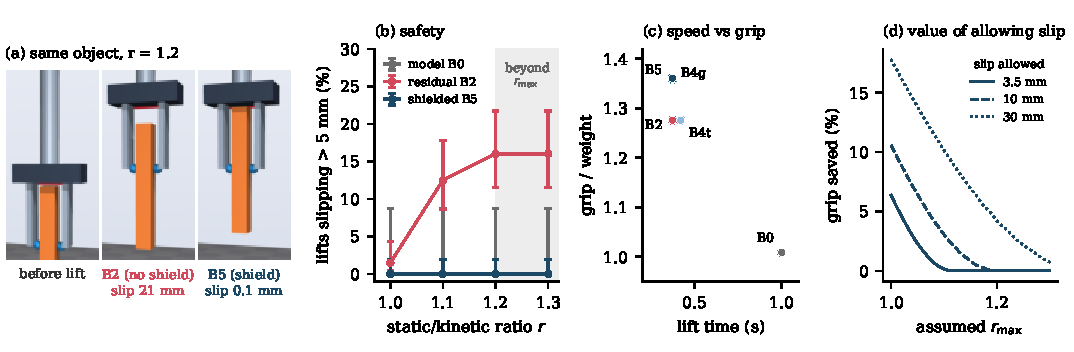
\includegraphics[width=\columnwidth]{fig_teaser.pdf}
\caption{Test set, 40 objects. Left: lifts that slipped more than 5\,mm (95\% Wilson intervals; residual methods pool
5 training seeds). The unshielded residual (B2) fails once kinetic friction is lower than static ($r>1$); the
shield-trained residual (B5) and the model controller (B0) never do, even beyond the shield's assumed $r_{\max}=1.2$.
Right: mean lift time and grip. All residual variants lift 2.7$\times$ faster than the model and grip harder; the
shield's price is a further 6\% grip (B4g, B5) or 13\% time (B4t).}\label{fig:teaser}
\end{figure}

\section{Introduction}
People lift objects with a grip only modestly above the force at which they would slip, scaled to the friction they
feel, and correct it reflexively when the object starts to slip \cite{johansson1984}. Robot grippers usually do the opposite:
they squeeze hard, because the object's weight and friction are unknown and a dropped object is costly. A light grip
matters for fragile, deformable or food items, and a fast lift matters for throughput. Slip detection and grip
stabilisation \cite{veiga2018,romeo2020} make light grips safer by reacting to slip, but reaction comes after the
fact.

In earlier work we studied a failure mode that makes light grips risky: when a grasped object breaks away, friction
drops from its static to its kinetic level, and a quasi-static model that ignores the drop under-predicts how far the
object travels \cite{aidoo2026b,aidoo2026c}. Physics shields, which project a learned action onto a set certified
by a friction model, prevented this in pivoting and controlled sliding \cite{aidoo2026c}. Lifting is the most common
grasp task and the natural next test, and it raises a question the earlier tasks did not: if a few millimetres of slip
are acceptable, can a policy deliberately allow them and gain a lighter or faster lift, with a certificate that the
slip stays small?

We answer this in simulation with a pre-registered study. Our contributions are:
\begin{itemize}\setlength\itemsep{1pt}
\item A closed-form slip bound for a lift at constant grip (Proposition~\ref{prop:lift}) that needs only a probed
breakaway grip and an assumed bound $r_{\max}$ on $\mu_s/\mu_k$, used as a shield that projects either the grip or
the lift duration.
\item Evidence (\Q1, \Q2) that an unshielded residual policy learns to exploit the quasi-static model's conservatism,
which is safe without a friction drop and fails 12--16\% of lifts with one; the shield removes every failure at a cost
of 6\% grip and no speed.
\item A comparison of grip and time projection (\Q3), certificate checks under $r_{\max}$ mismatch (\Q4), and an
exploratory analysis showing that the bound is a cliff: for $r_{\max}\ge1.1$ a slip allowance buys essentially no
grip. Lift-with-slip only pays when friction is known not to drop.
\end{itemize}

\section{Related Work}
\textbf{Grip force during lifting.} Johansson and Westling showed that humans set grip force to the object's friction
with a small safety margin, and correct it reflexively when slip begins \cite{johansson1984}. Robotic analogues detect
or predict slip with tactile sensing and raise the grip in response \cite{veiga2018}; Romeo and Zollo survey slip
detection methods and sensors \cite{romeo2020}. These approaches react to slip. We instead choose the grip and the
motion before the lift so that slip is bounded in advance, using only a probe of the breakaway grip.

\textbf{Residual learning and shields.} Residual policies learn corrections to a base controller
\cite{johannink2019,silver2018}. Shielding overrides unsafe actions using a model \cite{alshiekh2018}; safety
filters based on barrier functions and reachability generalise it \cite{ames2019,brunke2022}. Our previous paper
built shields from the static-to-kinetic friction transition for pivoting and sliding \cite{aidoo2026c}. Here the
transition happens during a commanded acceleration profile, the shield has two projection axes, and the task
explicitly tolerates some slip.

\textbf{Motion profiles and friction modelling.} We lift along a minimum-jerk trajectory \cite{flash1985}, which
fixes the peak acceleration for a given duration. Stick--slip is emulated in MuJoCo \cite{todorov2012} by switching the
friction coefficient, as in \cite{aidoo2026c}; richer friction models include rate dependence and pre-sliding
\cite{canudas1995}.

\section{Certified Lifting}\label{sec:method}
\begin{figure*}[t]\centering
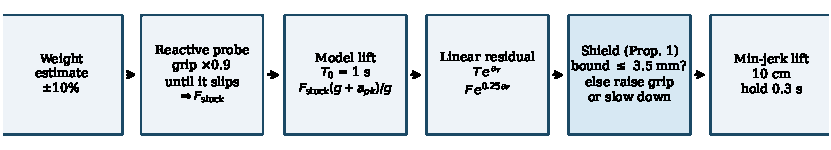
\includegraphics[width=\textwidth]{fig_method.pdf}
\caption{Episode pipeline. The probe and the model lift come from contact mechanics; the residual adjusts the lift time
and grip; the shield checks Proposition~\ref{prop:lift} and, if the slip bound exceeds 3.5\,mm, raises the grip
(grip axis) or lengthens the lift (time axis) until it does not, declining if neither suffices.}\label{fig:method}
\end{figure*}

\textbf{Task.} A parallel gripper holds a rod of mass $m\sim U[0.05,0.2]$\,kg and static friction $\mu_s\sim
U[0.4,0.8]$; kinetic friction is $\mu_k=\mu_s/r$ with $r$ unknown. The gripper lifts the rod 10\,cm along a
minimum-jerk profile of duration $T$, whose peak acceleration is $a_{pk}=5.77\,H/T^2$ \cite{flash1985}, at constant
grip $F$. A lift succeeds if the rod slips no more than $S_{\rm tol}=5$\,mm relative to the fingers.

\textbf{Probe.} With the palm still, the grip starts at $\hat m g/(2\cdot0.3)$ and is multiplied by 0.9 every 0.4\,s
until a slip monitor (noise 0.5\,mm) reads more than 2.5\,mm. The grip then snaps to $2.5\times$ the grip that moved,
within 20\,ms. $\Fs$, the last grip that held, is an upper bound on the breakaway grip at rest, so $g\,F/\Fs$ is a
lower bound on the static friction capacity per unit mass at grip $F$. The weight estimate $\hat m$ is within
$\pm10$\%.

\textbf{Model controller.} The quasi-static Coulomb lift uses $T_0=1$\,s and $F=\Fs(g+a_{pk})/g$: just enough static
friction at peak acceleration.

\begin{proposition}\label{prop:lift}
Let the palm follow an acceleration profile $a(t)$ at constant grip $F$, and let $r\le r_{\max}$. Slip cannot begin
while $g+a(t)\le gF/\Fs$. From the first instant $t_0$ where $g+a(t_0)>gF/\Fs$, define
$\bar a(t)=g+a(t)-gF/(r_{\max}\Fs)$, $\dot{\bar v}=\bar a$ with $\bar v$ clipped at 0, $\bar v(t_0)=0$. Then slip
during the profile is at most $\bar s=\int_{t_0}\bar v\,dt$.
\end{proposition}
\textit{Sketch.} The static capacity $2\mu_sF/m=gF/F_b\ge gF/\Fs$ since the true breakaway grip $F_b\le\Fs$. While
sliding, the kinetic capacity is $gF/(rF_b)\ge gF/(r_{\max}\Fs)$, so the rod's acceleration relative to the fingers is
at most $\bar a$; re-sticking only lowers it. Comparison of the two velocity equations gives $v\le\bar v$. \hfill$\square$

\textbf{Shield.} A command $(T,F)$ is certified if $\bar s\le s_{\lim}=S_{\rm tol}-1.5$\,mm, where 1.5\,mm is a
sensing margin; $\bar s$ is evaluated over the 0.6\,s grip ramp and settle, the lift and a 0.3\,s hold. The
\emph{grip projection} raises $F$ to the smallest certified grip; the \emph{time projection} lengthens $T$ to the
shortest certified duration (up to 2\,s). If neither exists the shield declines and the model's lift is used.
We use $r_{\max}=1.2$.

\textbf{Residual policy.} A linear policy maps six probe features (log breakaway grip over weight, probe resolution,
weight, probe count, grip scale, bias) through $\tanh$ to $(a_T,a_F)\in[-1,1]^2$, setting $T=T_0e^{a_T}$ (clipped to
[0.25,\,2]\,s) and $F=F_{\rm model}(T)\,e^{0.25a_F}$. The reward is $-10$ for a failed lift and otherwise
$-T/T_0-0.1\,F/(mg)$.

\section{Experimental Setup}\label{sec:setup}
\textbf{Simulation.} MuJoCo 3 at 1\,ms, palm driven kinematically along a vertical slide, spherical pads with
elliptic cones and no-slip iterations, rod on a vertical slide joint (a free rod rocked about the grasp axis after
slip; we study axial slip only). Friction switches to $\mu_k$ when the relative speed exceeds 2\,cm/s and back below
2\,mm/s. Before any training we validated the rig (Table~\ref{tab:val}). The static breakaway grip matched
$mg/(2\mu)$ to within 1.1\%. During lifts the quasi-static model over-predicted the grip needed by 2--11\%, more at
short $T$. In 120 random lifts no lift with a bound of zero slipped beyond elastic creep (at most 0.2\,mm over the bound),
and none with a bound under 5\,mm slipped more than 5\,mm.

\begin{table}[t]\centering\footnotesize
\caption{Rig validation (development objects only).}\label{tab:val}
\begin{tabular}{@{}lr@{}}\toprule
Check & Result\\\midrule
Static breakaway / $mg/(2\mu)$ ($n=20$) & 0.989 (0.986--1.014)\\
Lift breakaway / $m(g+a_{pk})/(2\mu)$, $T=0.25$ / 0.5 / 1\,s & 0.890 / 0.952 / 0.983\\
Lifts with zero bound that slipped ($n=67$) & 0\\
Max excess of slip over a non-zero bound & 0.20\,mm\\
Lifts $>5$\,mm with bound $\le5$\,mm ($n=120$) & 0\\
Elastic creep at grip margin 1.1--2.0 & 0.09--0.19\,mm\\\bottomrule
\end{tabular}\end{table}

\textbf{Methods.} B0: model controller. B0S: model with the grip shield. B2: residual trained and tested without a
shield. B4g, B4t: B2's weights with the grip or time shield at test only. B5: residual trained and tested with the grip
shield. Residuals were trained with antithetic evolution strategies as in \cite{aidoo2026c} (6 pairs, 6 objects per
iteration, $\sigma=0.1$, Adam step 0.06, 20 iterations, 1{,}560 episodes per run), 5 seeds each, on $r\sim
U[1.0,1.2]$, starting from zero weights, i.e.\ from the model controller.

\textbf{Evaluation and statistics.} Test set: 40 new objects, each at $r\in\{1.0,1.1,1.2,1.3\}$. Confirmation set:
40 further objects with $r\sim U[1.0,1.3]$, run once after the test results were committed. Learned methods are
averaged over seeds per object; differences from B0 use paired Wilcoxon tests (lift time, grip) and exact McNemar
tests (objects with any failure), Holm-corrected, with hierarchical bootstrap 95\% intervals (seeds, then objects).
The protocol was committed before training; three dated deviations are recorded in it (Section~\ref{sec:lim}).

\section{Results}
\begin{table}[t]\centering\footnotesize
\caption{Test set, $r_{\max}=1.2$. Lift time and grip are means over all lifts (they do not depend on $r$);
failures are lifts with slip $>5$\,mm out of 200 (40 for B0, B0S). None of the failures dropped the rod.}\label{tab:main}
\setlength{\tabcolsep}{3.6pt}
\begin{tabular}{@{}lccccccc@{}}\toprule
 & $T$ (s) & $F/mg$ & \multicolumn{4}{c}{failures at $r=$} & max slip\\
 & & & 1.0 & 1.1 & 1.2 & 1.3 & (mm)\\\midrule
B0 model & 1.000 & 1.009 & 0 & 0 & 0 & 0 & 0.49\\
B0S model+shield & 1.000 & 1.009 & 0 & 0 & 0 & 0 & 0.49\\
B2 residual & 0.372 & 1.276 & 3 & 25 & 32 & 32 & 56.0\\
B4g test shield, grip & 0.372 & 1.358 & 0 & 0 & 0 & 0 & 0.12\\
B4t test shield, time & 0.420 & 1.276 & 0 & 0 & 0 & 0 & 0.14\\
B5 trained shield & 0.370 & 1.361 & 0 & 0 & 0 & 0 & 0.11\\\bottomrule
\end{tabular}\end{table}

\subsection*{\Q1: How much faster, and at what grip?}
Every residual variant lifted 2.7 times faster than the model: B5 cut the lift time by 0.630\,s (95\% CI
0.629--0.630; Holm $p<10^{-10}$ at every $r$), from 1.00 to 0.37\,s (Table~\ref{tab:main}). All ten policies ended at
the same corner, $a_T=-1$, the edge of the action range, so the speed gain is set by our action bound, not by the
physics. Faster lifts need more grip, because peak acceleration grows as $1/T^2$: B5 gripped 0.352\,$mg$ harder than
the model (CI 0.330--0.374), 35\% more. The unshielded residual gripped less, $+0.267\,mg$, because it set the grip
on average 6\% (range $-11$\% to $+3$\%) below the model's grip for its own lift time. Lift time is not the whole
episode: the probe took a median of 4.1\,s (7.5 probe steps), so the end-to-end episode is about 10\% shorter.

\subsection*{\Q2: Does the residual stay safe as friction drops?}
No. B2's grip cut works when $r=1$ (3 failures in 200 lifts), because the quasi-static model over-predicts the grip
needed at short lift times by about 8\% (Table~\ref{tab:val}) and the probe's 0.9 step adds margin. When the rod does
start to slip, kinetic friction is too low to stop it: failures rose to 25, 32 and 32 of 200 at $r=1.1$, 1.2 and
1.3, with slips up to 56\,mm. Per object, B2 failed on 14 objects where the model did not at $r=1.1$ and 16 at
$r=1.2$ and 1.3, never the reverse (Holm $p=0.001$ and $p=0.0004$). How much each seed cut differed widely: at
$r=1.2$ the five B2 policies failed 2, 6, 14, 2 and 8 times in 40. All shielded methods had zero failures at every
$r$. On the confirmation set B2 failed 35 of 200 lifts (1, 16 and 18 in the $r$ bands $(1,1.1]$, $(1.1,1.2]$ and
$(1.2,1.3]$; 15 objects worse than the model, none better, $p=6\times10^{-5}$), while B4g and B5 failed none, with the
same speed (0.371\,s, 0.370\,s) and grip ($+0.32\,mg$) as on the test set.

\subsection*{\Q3: Raise the grip or slow the lift?}
Applied to the same B2 commands, both projections intervened on 95.5\% of lifts and removed every failure. The grip
projection kept B2's speed and added 6.4\% grip ($1.358$ vs $1.276\,mg$); the time projection kept B2's grip and
slowed the lift by 13\% (0.420 vs 0.372\,s). Under our reward, which values 1\,s of lift time like 10\,$mg$ of grip,
the grip projection is better, and training with it in the loop (B5) gave the same result as adding it at test time
(B4g): 0.370 vs 0.372\,s and 1.361 vs 1.358\,$mg$. The shield never declined.

\begin{figure}[t]\centering
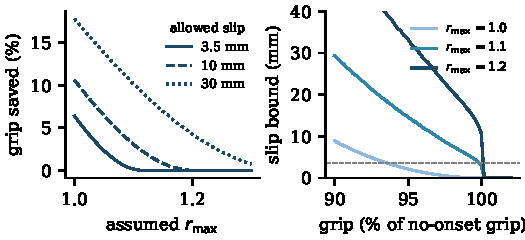
\includegraphics[width=\columnwidth]{fig_cliff.pdf}
\caption{Exploratory: why a slip allowance buys little. Left: grip saved by allowing 3.5, 10 or 30\,mm of slip, at
$T=0.37$\,s, relative to the grip at which slip never starts, as a function of the assumed $r_{\max}$. Right: the slip
bound against grip. With $r_{\max}=1$ the bound grows gradually as grip falls; with a friction drop it jumps to
centimetres as soon as slip can begin.}\label{fig:cliff}
\end{figure}

\subsection*{\Q4: Does the certificate hold, and what if $r_{\max}$ is wrong?}
Every certified lift at $r_{\max}=1.2$ had a slip bound of exactly zero: the shield placed the grip at the point where
slip cannot start. Measured slip was 0.05--0.49\,mm, which is elastic creep in the pads, not friction slip; it
exceeds a zero bound, so the pre-registered ``exceedance'' rate is 100\%, but the largest excess is a third of the
1.5\,mm margin and no certified lift came within 4.5\,mm of the tolerance (0 of 2{,}560 at $r_{\max}=1.2$, including
640 lifts at $r=1.3>r_{\max}$, and 0 of 960 at $r_{\max}=1.4$). Lifts beyond $r_{\max}$ were safe because slip never
started, so the kinetic level never mattered. Underestimating the drop was not safe: with $r_{\max}=1.0$ the shield
let B5 grip 6.4\% less (1.274\,$mg$), and 60 of its 600 lifts at $r>1$ slipped more than 5\,mm (10, 25 and 25 at
$r=1.1$, 1.2, 1.3; worst excess over the bound 18\,mm), against 0 of 200 at $r=1$.

The exploratory analysis in Fig.~\ref{fig:cliff} explains this. Allowing 3.5\,mm of slip saves 6.4\% grip if
friction does not drop, 2.3\% if it may drop by 5\%, 0.15\% at 10\% and nothing from 15\%; allowing 10\,mm saves
nothing from $r_{\max}=1.2$. Once slip starts, the kinetic deficit $(g+a)(1-1/r_{\max})$ acts for the rest of the
acceleration phase, so the slip is either zero or large. The ratio of certified grip to the no-onset grip was the same
for all 40 test objects, since it depends only on $r_{\max}$ and $T$.

\section{Limitations}\label{sec:lim}
All results are from simulation. Stick--slip is emulated by switching the friction coefficient, with thresholds we
tuned; real contacts show rate-dependent friction, pre-sliding and pad wear \cite{canudas1995}, and the rod was
constrained to slide axially. The certificate assumes $\Fs$ bounds the breakaway grip during the lift, which held here
because the quasi-static model is conservative at short $T$ (Table~\ref{tab:val}); on hardware this needs checking.
The residual's speed gain is bounded by its action range, and the lift is a small part of an episode dominated by a
4\,s probe; a faster probe is the larger opportunity. Three deviations from the protocol are recorded in it: the
exceedance metric counts elastic creep (we also report the size of the excess); the confirmation set, whose $r$ varies
per object, was analysed pooled; and the slip-allowance analysis was exploratory. Training used 1{,}560 episodes and
linear policies; richer policies might find other trade-offs.

\section{Conclusion}
A learned lift policy, given the freedom to grip lighter than a friction model, learned to exploit the model's
conservatism, which is harmless only when friction does not drop on breakaway. A closed-form slip bound used as a
shield removed every failure in simulation, at 6\% extra grip and no loss of speed, even beyond its assumed friction
drop. Allowing a little slip turned out to be worth little: with a friction drop of 10\% or more, the only certified
lifts are those in which slip never starts. The next steps are hardware validation of the probe and the bound, and a
faster probe.

\section*{Data Availability}
Code, protocol with deviations, per-episode results and the scripts behind every number:
\url{https://github.com/CAN-Aidoo/lift-shield}.

\section*{Use of AI Tools}
Code, analysis and drafting were carried out with the assistance of an AI model (Claude, Anthropic) under the author's
direction. The author takes responsibility for the content.

\balance
\footnotesize
\begin{thebibliography}{99}\setlength{\itemsep}{0pt}
\bibitem{johansson1984} R.~S. Johansson and G.~Westling, ``Roles of glabrous skin receptors and sensorimotor memory in automatic control of precision grip when lifting rougher or more slippery objects,'' \emph{Exp. Brain Res.}, 56(3):550--564, 1984.
\bibitem{veiga2018} F.~Veiga, B.~Edin, and J.~Peters, ``Grip stabilization through independent finger tactile feedback control,'' \emph{Sensors}, 20(6):1748, 2020.
\bibitem{romeo2020} R.~A. Romeo and L.~Zollo, ``Methods and sensors for slip detection in robotics: a survey,'' \emph{IEEE Access}, vol.~8, 2020.
\bibitem{aidoo2026b} C.~Aidoo, ``Residual learning on a physics pivoting controller: faster search, and where the quasi-static model breaks,'' engrXiv, doi:10.31224/8542, 2026.
\bibitem{aidoo2026c} C.~Aidoo, ``Physics guards for residual policies at breakaway: when learned corrections should defer to a friction model,'' engrXiv, doi:10.31224/8603, 2026.
\bibitem{johannink2019} T.~Johannink, S.~Bahl, A.~Nair, J.~Luo, A.~Kumar, M.~Loskyll, J.~A. Ojea, E.~Solowjow, and S.~Levine, ``Residual reinforcement learning for robot control,'' in \emph{Proc. IEEE ICRA}, 2019, arXiv:1812.03201.
\bibitem{silver2018} T.~Silver, K.~Allen, J.~Tenenbaum, and L.~Kaelbling, ``Residual policy learning,'' arXiv:1812.06298, 2018.
\bibitem{alshiekh2018} M.~Alshiekh, R.~Bloem, R.~Ehlers, B.~K{\"o}nighofer, S.~Niekum, and U.~Topcu, ``Safe reinforcement learning via shielding,'' in \emph{Proc. AAAI}, 2018, arXiv:1708.08611.
\bibitem{ames2019} A.~D. Ames, S.~Coogan, M.~Egerstedt, G.~Notomista, K.~Sreenath, and P.~Tabuada, ``Control barrier functions: theory and applications,'' in \emph{Proc. ECC}, 2019, arXiv:1903.11199.
\bibitem{brunke2022} L.~Brunke, M.~Greeff, A.~W. Hall, Z.~Yuan, S.~Zhou, J.~Panerati, and A.~P. Schoellig, ``Safe learning in robotics: from learning-based control to safe reinforcement learning,'' \emph{Annu. Rev. Control Robot. Auton. Syst.}, 2022, arXiv:2108.06266.
\bibitem{flash1985} T.~Flash and N.~Hogan, ``The coordination of arm movements: an experimentally confirmed mathematical model,'' \emph{J. Neurosci.}, 5(7):1688--1703, 1985.
\bibitem{todorov2012} E.~Todorov, T.~Erez, and Y.~Tassa, ``MuJoCo: a physics engine for model-based control,'' in \emph{Proc. IEEE/RSJ IROS}, 2012, pp.~5026--5033.
\bibitem{canudas1995} C.~Canudas de Wit, H.~Olsson, K.~J. {\AA}str{\"o}m, and P.~Lischinsky, ``A new model for control of systems with friction,'' \emph{IEEE Trans. Autom. Control}, 40(3):419--425, 1995.
\end{thebibliography}
\end{document}
